\section{Diagramme}


Bevor wir mit der Implementation des Projektes starten, 
führten wir ein Gruppen Brainstorming durch um festzulegen, 
welche Aufgabe jeder einzelne für das Projekt erfüllen muss. 



\subsection{Requirements}

Das Ergebnis des Brainstormings verfasste jeder in einer Requirements Tabelle zusammen, um später zu verhindern das Probleme zwischen den einzelnen Clients auftreten können.


So wurde festgelegt das jeder Client seine eigene ID und Namen besitzt. 


Zudem sind alle Clients mit dem Server verbunden, dort können sie sich mit ihrem eigenen Namen anmelden.


Ein weiterer Ansatz ist es das jeder Client, Nachrichten Senden und Empfangen kann. 


So sollen die Standorte oder Aufgaben zum Server gesendet und dort verarbeitet werden.


Die Nachrichten sollen innerhalb von 5 Sekunden zwischen den Clients ausgetauscht werden.


Zum Schluss wurde festgelegt das jeder sein Programm mit Python programmieren soll um später alles reibungslos zusammenfassen zu können.


\begin{figure}[htbp] 
  \centering
     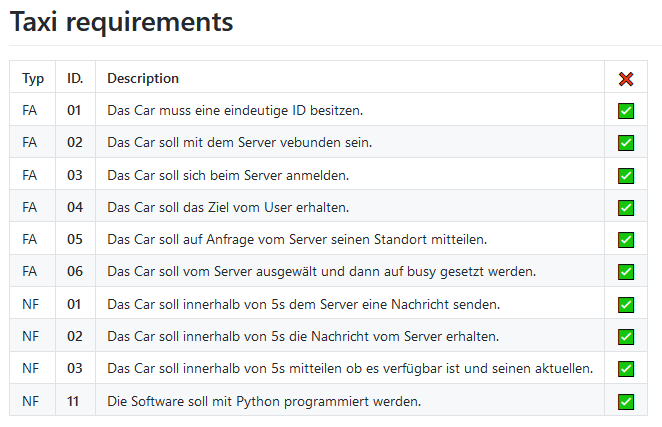
\includegraphics[width=0.48\textwidth]{Bsp_requirments.png}
     \caption{Requirments}
\end{figure}




\subsection{Use-Case}

Der Nächste Schritt im Projekt ist, aus dem gesammelten Informationen der Requirements, Use-Case Diagramme für jeden Client zu erstellen.


Use-Case Diagramme verdeutlichen die 
Aufgaben und 

Verbindungen zwischen den einzelnen Clients.


So ist der Server mit jedem Client verbunden, vorab Registrieren sich alle Clients beim Server. 


Nun bekommt der Server eine Message vom User, 'request car'.
Folgend wird 'select closest car' vom Server durchgeführt und dem nächsten Car mitgeteilt das er zum anfragendem User fahren muss. 


Der Server setzt das bestellte Car auf Busy, 'change car status'.


Danach erhält das Car eine Message vom User mit den Wunsch Zielort und fährt dort hin.


Am Zielort setzt der User dann das Car beim Server wieder auf free.


Zum Schluss erfragt der Server den neuen Standort des Cars und schließt die Handlung damit ab.



\begin{figure}[htbp] 
  \centering
     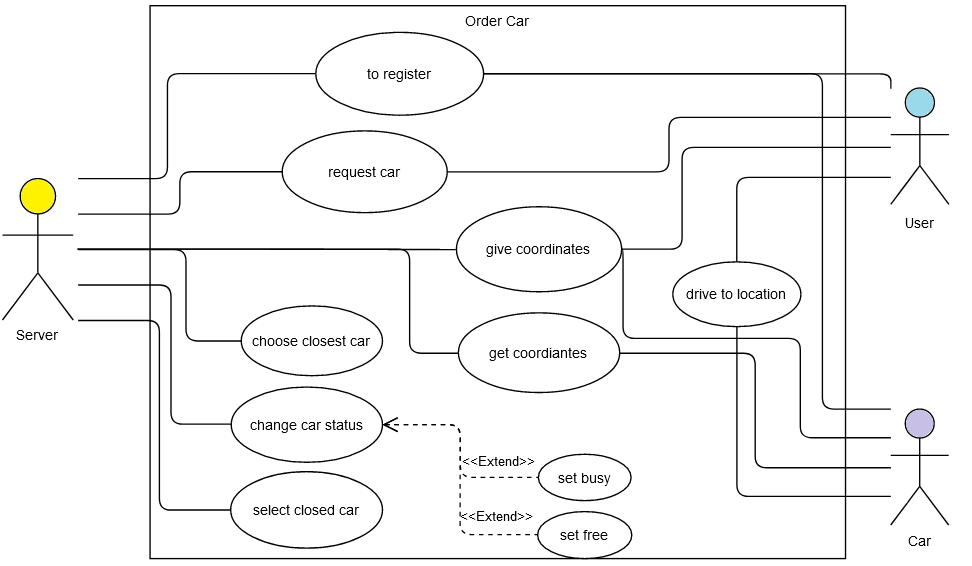
\includegraphics[width=0.48\textwidth]{Use-Case_Server.png}
     \caption{Use-Case}
\end{figure}


